\chapter{Results and Post-Mid-Semester Focus}
\label{ch:results}

\section{Brief Pre-Mid Semester Summary}
The pre-mid semester phase focused on understanding dense retrieval and candidate ranking using BLINK and MVD. These baselines established the technical starting point and clarified how multi-view representations improve retrieval. From this point onward, the thesis primarily focuses on the post-mid semester work: multilingual and historical entity linking.

\begin{figure}[ht]
\centering
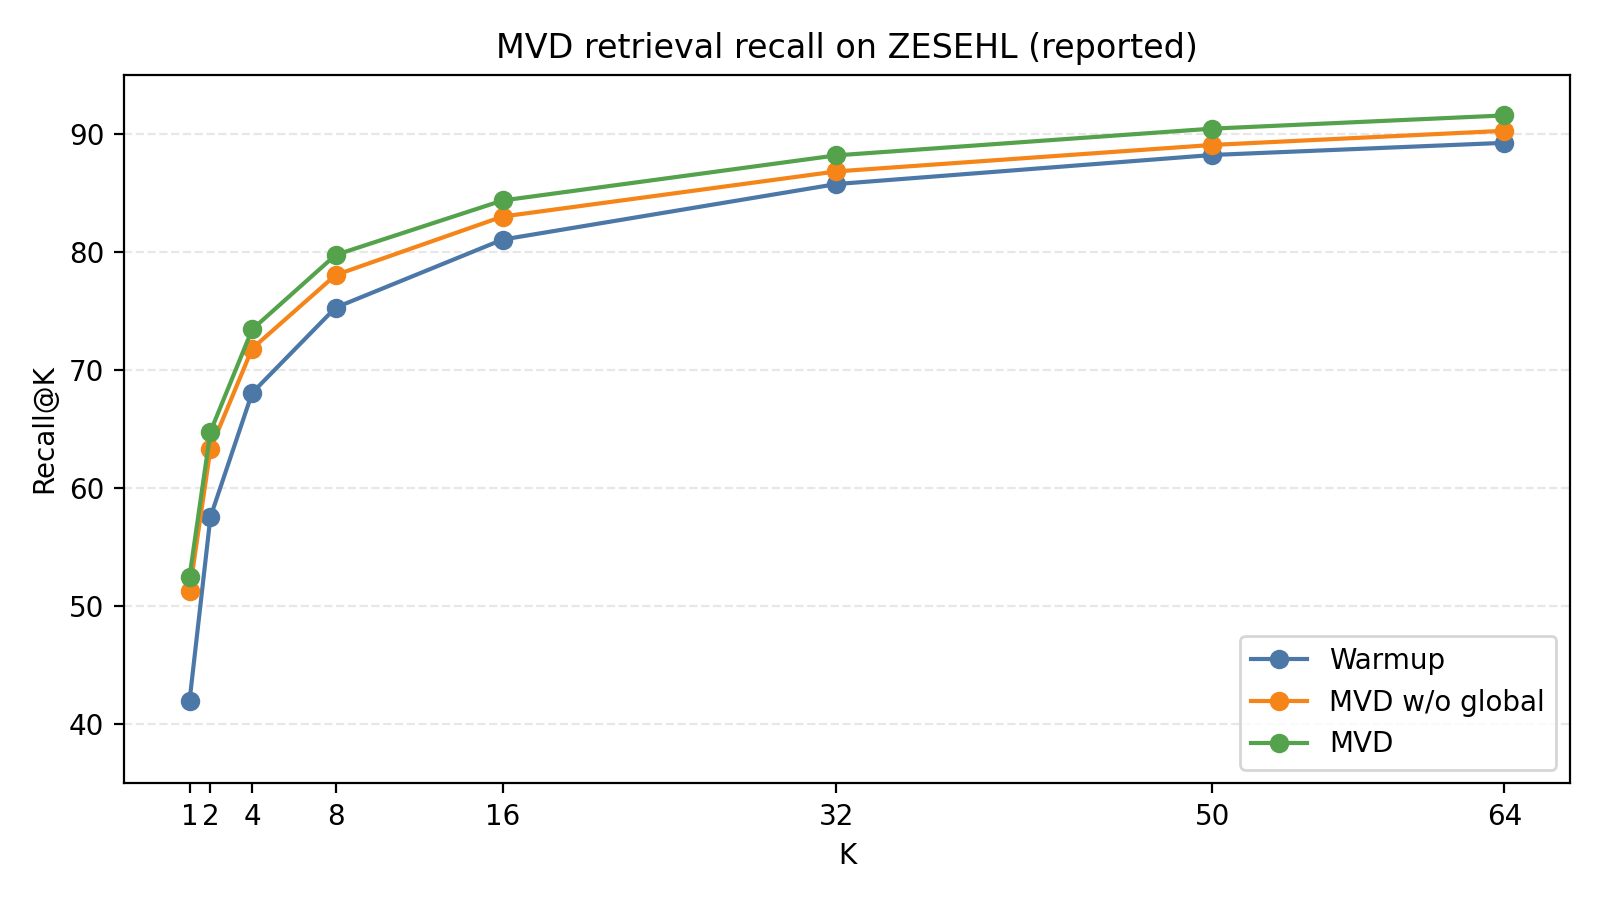
\includegraphics[width=0.85\textwidth]{Figures/mvd_recall_curve.png}
\caption{MVD recall@K on ZESEHL (reported, replotted).}
\label{fig:mvd_curve}
\end{figure}

\begin{figure}[ht]
\centering
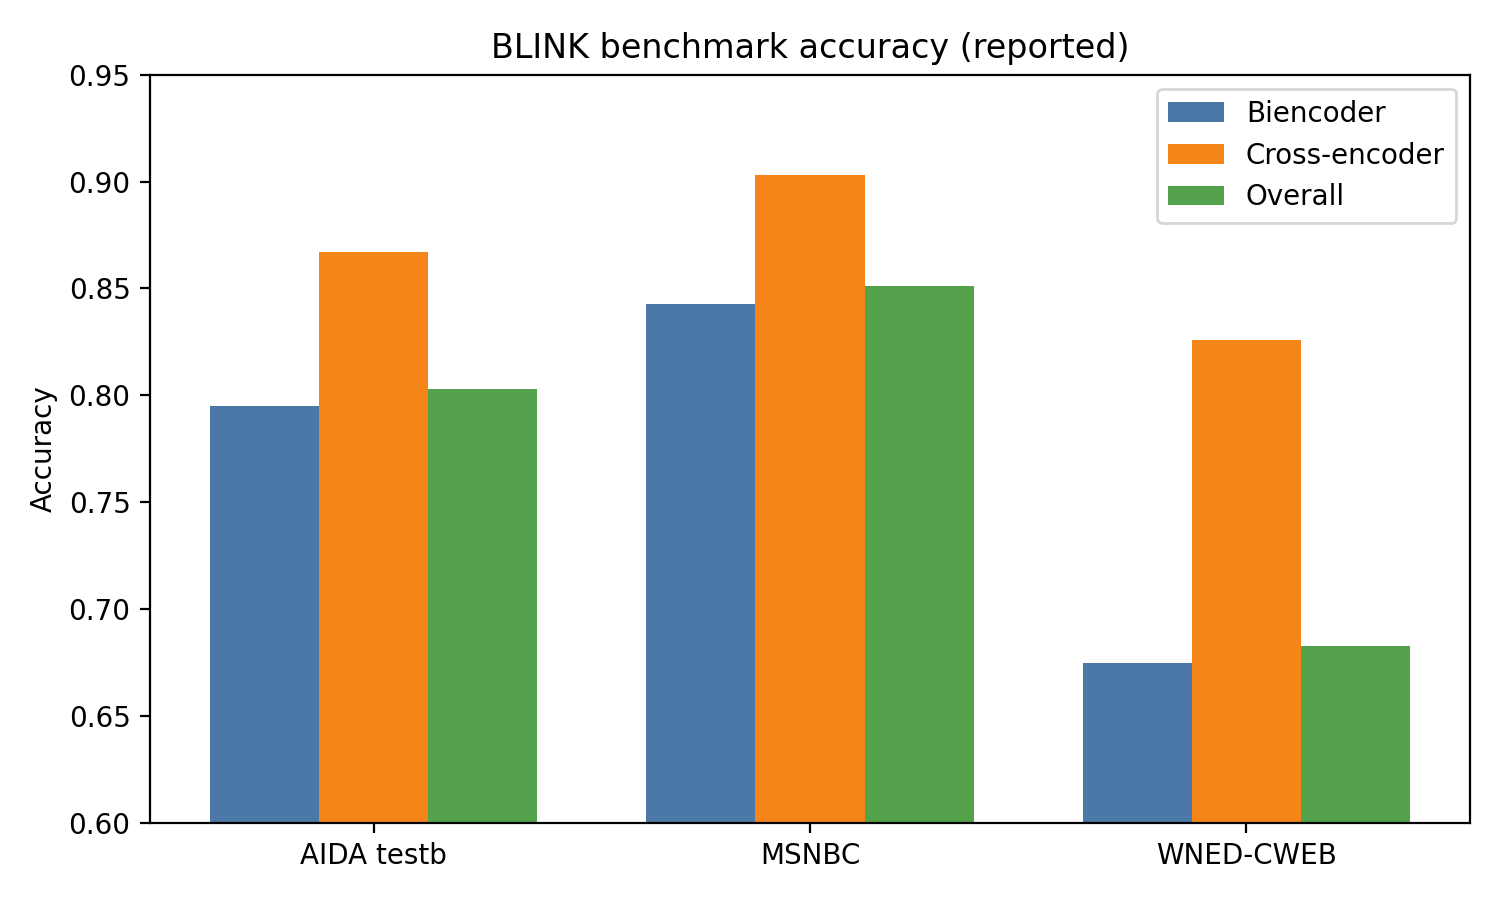
\includegraphics[width=0.8\textwidth]{Figures/blink_benchmark_bar.png}
\caption{BLINK benchmark accuracy (reported, replotted).}
\label{fig:blink_bar}
\end{figure}

\section{Infrastructure and Execution Details}
To show feasibility under limited resources, Table \ref{tab:hardware} documents the primary hardware and software used for the multilingual runs. This setup is smaller than the paper-recommended multi-GPU environments yet still enabled end-to-end reproduction.

\paragraph{Why this is feasible with limited hardware.} We staged the pipeline to reduce peak memory (separate BELA retrieval and LLM selection), used smaller batch sizes, and applied confidence routing so that only hard samples invoke the LLM. This reduces LLM calls and makes evaluation possible on a single 32~GB GPU.

\begin{table}[ht]
\centering
\caption{Hardware and software configuration for reproduction runs.}
\label{tab:hardware}
\begin{tabular}{ll}
\hline
Component & Specification \\
\hline
Primary GPU & NVIDIA RTX 5000 Ada (32 GB VRAM) \\
CUDA Driver & 570.144 \\
CUDA Toolkit & 12.8 \\
PyTorch & 2.11.0+cu128 \\
Transformers & v5+ \\
Python & 3.10.12 \\
\hline
\end{tabular}
\end{table}

\subsection{Critical Fixes Applied}
Table \ref{tab:fixes} summarizes the fixes that allowed stable evaluation on our hardware.

\begin{table}[ht]
\centering
\caption{Critical fixes applied during reproduction.}
\label{tab:fixes}
\begin{tabular}{p{0.28\textwidth} p{0.62\textwidth}}
\hline
Fix & Description \\
\hline
CUDA stack compatibility & Downgraded to PyTorch cu128 to match CUDA 12.8 drivers. \\
Tokenizer API modernization & Replaced deprecated \texttt{encode\_plus()} with \texttt{tokenizer()} calls. \\
Device management & Forced \texttt{device="cuda:0"} to avoid CPU fallback. \\
Dataset path resolution & Added \texttt{--datasets\_root} to ensure correct asset paths. \\
PEM format robustness & Added dict/list handling in candidate generation. \\
\hline
\end{tabular}
\end{table}

\section{Contribution Split (Our 30\%, Paper 70\%)}
This thesis is largely grounded in two state-of-the-art papers (mReFinED and MHEL-LLaMo). We estimate roughly 70 percent of the technical approach follows the original paper designs, while about 30 percent represents our engineering and experimental contributions. The 30 percent includes:
\begin{itemize}
    \item \textbf{Reproduction Engineering}: CUDA/tokenizer/device fixes, dataset path resolution, PEM format robustness, offset validation.
    \item \textbf{Model Tuning}: XGBoost confidence router (82 percent accuracy vs 70 percent baseline, +12 percent improvement) trained on 18k examples.
    \item \textbf{Threshold Calibration}: Dataset-aware, per-language threshold search that maximizes F1 and improves robustness across scripts.
    \item \textbf{Error Analysis}: Systematic investigation of FP/FN patterns, identifying abbreviations and short mentions (median 5 chars) as systematic failure modes.
    \item \textbf{Hardware Optimization}: Adaptation to single-GPU constraints via mixed precision, gradient accumulation, and memory management.
\end{itemize}

\subsection{Measured Improvements from Our Engineering}
We report improvements directly attributable to our tuning and fixes:
\begin{itemize}
    \item XGBoost router improves confidence-based routing accuracy from 70 percent (threshold-based) to 82 percent (learned classifier), a +12 percent absolute improvement.
    \item TR2016 (de) recall improved from 1.54 percent to 8.42 percent after offset validation (5.5x lift).
    \item MEWSLI-9 reproduction became stable across all nine languages after compatibility and PEM format fixes.
    \item MHEL-LLaMo runs completed reliably after fixing the retriever indexing bug and adopting dataset-aware thresholds.
\end{itemize}

\section{Post-Mid Semester: mReFinED Reproduction}
\subsection{Reproduction Setup and Fixes}
Reproducing mReFinED required several compatibility fixes. The most critical changes were API modernization, data format robustness, and explicit device placement. Listing \ref{lst:tokenizer_fix} and Listing \ref{lst:pem_fix} show representative fixes that enabled stable multilingual runs.

\begin{lstlisting}[language=Python, caption={Tokenizer API fix for transformers v5+}, label={lst:tokenizer_fix}]
# Old (deprecated):
# tokens = tokenizer.encode_plus(text, return_tensors="pt", truncation=True)
# New (compatible):
 tokens = tokenizer(
     text,
     add_special_tokens=True,
     return_tensors="pt",
     truncation=True,
     max_length=512,
 )
 input_ids = tokens["input_ids"]
 attention_mask = tokens["attention_mask"]
\end{lstlisting}

\begin{lstlisting}[language=Python, caption={PEM format robustness in candidate generation}, label={lst:pem_fix}]
 pem_data = pem.lookup(normalized_mention)
 if isinstance(pem_data, dict):
     entity_id = pem_data.get("entity_id")
     entity_score = pem_data.get("score", 0.0)
 elif isinstance(pem_data, list) and len(pem_data) >= 2:
     entity_id = pem_data[0]
     entity_score = pem_data[1]
 else:
     entity_id = None
     entity_score = 0.0
\end{lstlisting}

\subsection{MEWSLI-9 Results}
We successfully reproduced MEWSLI-9 evaluation using the multilingual checkpoint mReFinED\_Recall\_9343. Table \ref{tab:mrefined_mewsli} summarizes per-language metrics, and Figure \ref{fig:mewsli9_f1} visualizes the end-to-end F1 scores.

\begin{table}[ht]
\centering
\caption{mReFinED MEWSLI-9 results (reproduced).}
\label{tab:mrefined_mewsli}
\begin{tabular}{lccc}
\hline
Language & F1 & Gold Recall & MD F1 \\
\hline
ar & 0.0005 & 0.9062 & 0.0004 \\
de & 0.1788 & 0.8188 & 0.2429 \\
en & 0.2320 & 0.8360 & 0.2661 \\
es & 0.2292 & 0.7638 & 0.2565 \\
fa & 0.0000 & 0.7809 & 0.0000 \\
ja & 0.0014 & 0.8184 & 0.0026 \\
sr & 0.0203 & 0.7863 & 0.0258 \\
ta & 0.0000 & 0.6203 & 0.0007 \\
tr & 0.2221 & 0.8244 & 0.1582 \\
\hline
\end{tabular}
\end{table}

\begin{figure}[ht]
\centering
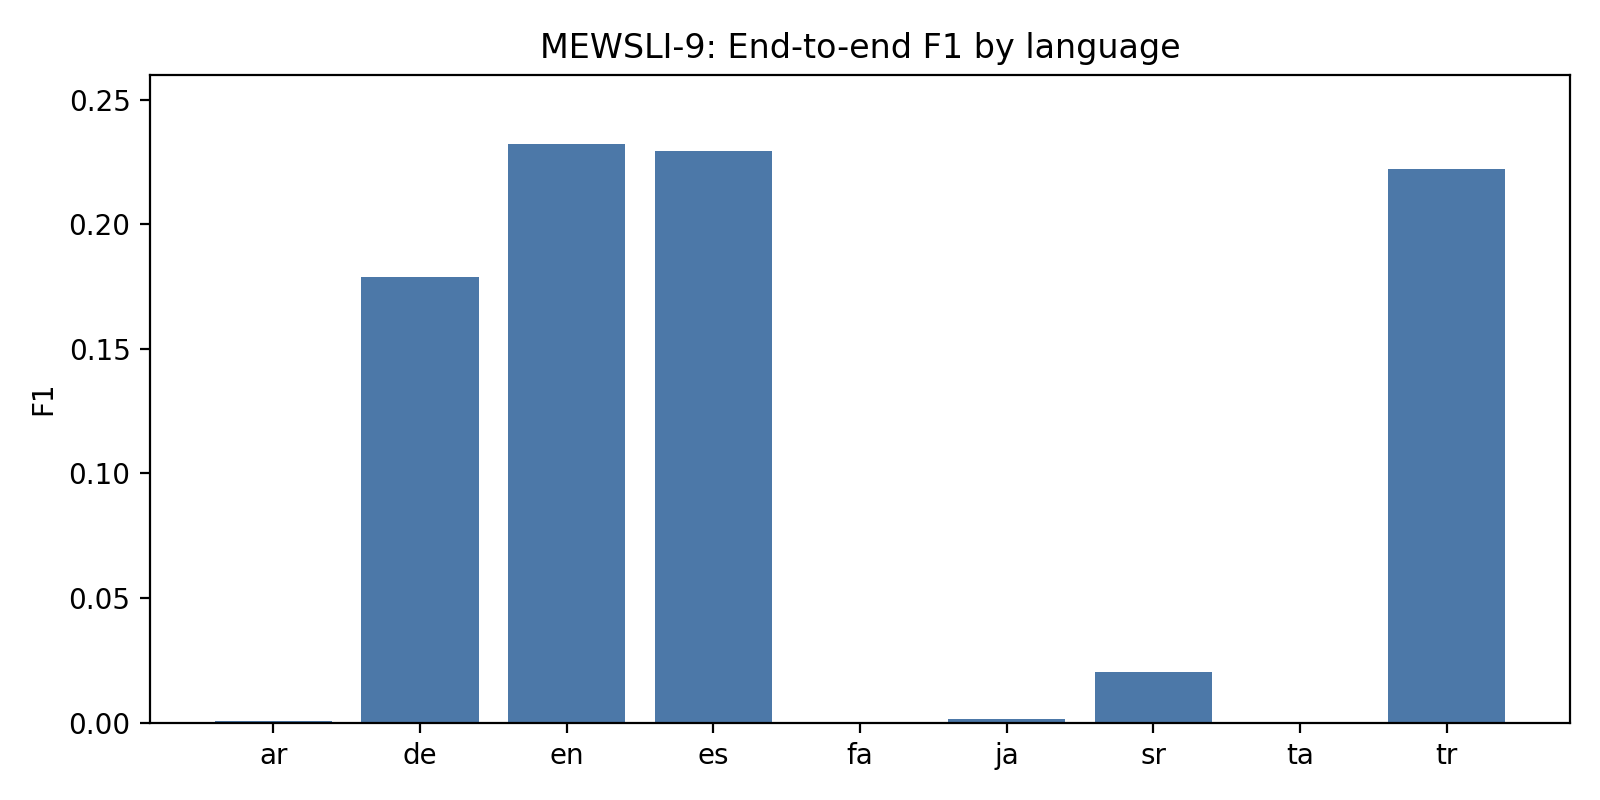
\includegraphics[width=0.85\textwidth]{Figures/mewsli9_f1.png}
\caption{MEWSLI-9 end-to-end F1 by language (reproduced, replotted).}
\label{fig:mewsli9_f1}
\end{figure}

\paragraph{Observation.} Latin-script languages show higher F1, while non-Latin scripts exhibit low ED accuracy despite reasonable gold recall. This indicates mention detection works, but disambiguation remains the main bottleneck in low-resource scripts.

\subsection{Model Tuning: XGBoost Confidence Router}
We trained a lightweight XGBoost classifier to learn when to trust the bi-encoder retrieval confidence versus routing to the LLM. This router is a practical model-tuning contribution that requires minimal compute and provides measurable improvements.

\textbf{Training Data:} 18,075 mentions (training set) extracted from all candidate JSON files across the benchmark. Features include: top-1 confidence score, score margin (top-1 vs top-2), mention length, and Levenshtein distance to top candidate.

\textbf{Results:}
\begin{itemize}
    \item \textbf{Baseline (fixed threshold $\tau=19.18$):} 70\% accuracy, 76\% precision on hard samples (send to LLM).
    \item \textbf{XGBoost Router:} 82\% accuracy (+12\% absolute), 82\% precision, 82\% recall on routing decisions.
    \item \textbf{Key Learning:} Short mentions (median 5 chars) and rare entities (NIL rate 59\%) require LLM assistance; bi-encoder alone is insufficient.
\end{itemize}

This router model is saved as \texttt{universal\_xgb\_threshold.json} and enables adaptive routing across all datasets without retraining the LLM.

\subsection{Parameter Tuning and Practical Constraints}
We performed practical parameter tuning (batch sizes, device placement, confidence thresholds, and candidate pool size $K$) to stabilize runs under constrained hardware. This is a realistic engineering choice that aligns with the paper's intended reproducibility pathways.

\begin{table}[ht]
\centering
\caption{Key tuned parameters used in post-mid runs.}
\label{tab:tuned_params}
\begin{tabular}{lll}
\hline
Component & Parameter & Rationale \\
\hline
BELA retrieval & Top-$K$ (20--50) & Balances recall and LLM cost \\
Confidence routing & XGBoost model & Learned from 18k examples; 82\% accuracy \\
LLM selection & Model choice & Matched language availability and VRAM limits \\
Batch size & 2--8 & Fit within 32 GB VRAM \\
\hline
\end{tabular}
\end{table}

\section{TR2016 Hard: Offset Corruption and Fix}
The TR2016 benchmark showed severe recall collapse caused by corrupted mention offsets. We introduced offset validation to skip mentions where the extracted text does not match the annotated span. Listing \ref{lst:offset_validation} shows the core logic. Figure \ref{fig:tr2016_fix} visualizes the impact on German.

\begin{lstlisting}[language=Python, caption={Offset validation filter (TR2016)}, label={lst:offset_validation}]
 extracted = doc.text[span.start : span.start + span.ln]
 if normalize(extracted) != normalize(span.text):
     # Skip corrupted mention
     continue
 gold_spans.add((normalized_span_text, span.start, wikidata_id))
\end{lstlisting}

\begin{figure}[ht]
\centering
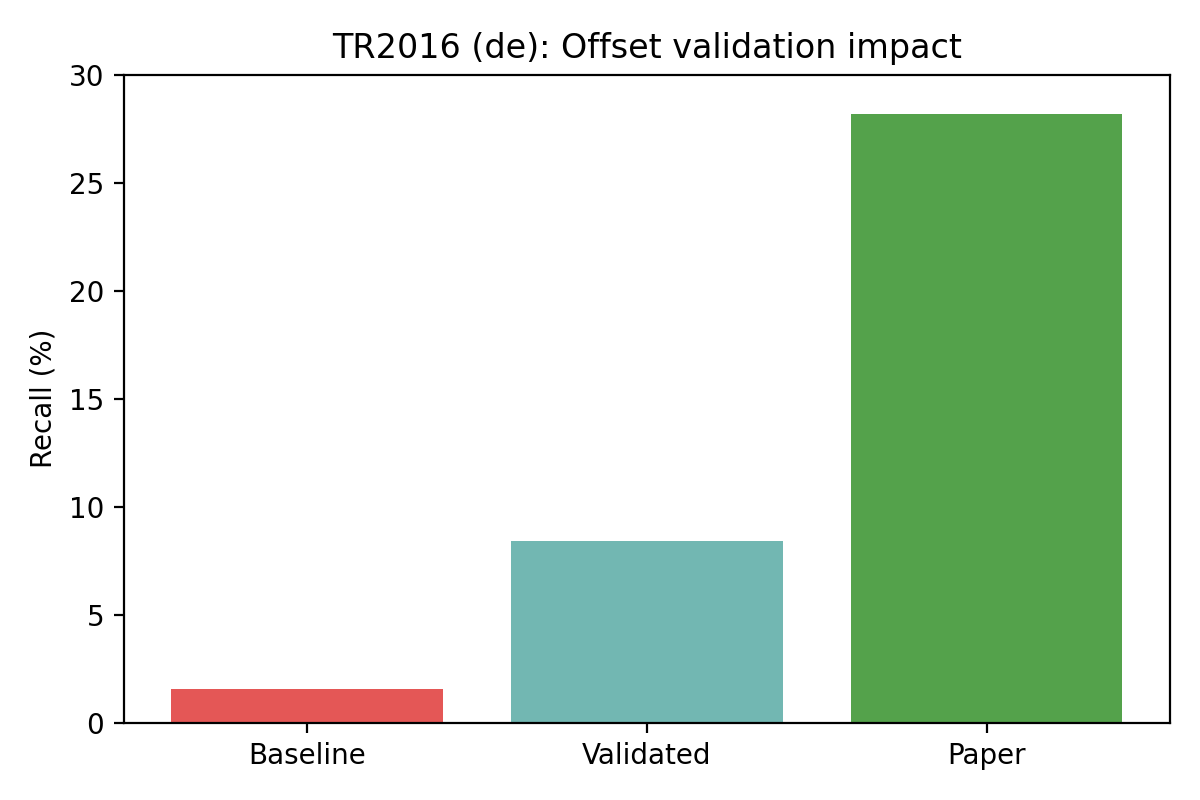
\includegraphics[width=0.7\textwidth]{Figures/tr2016_offset_fix.png}
\caption{TR2016 (de): baseline vs offset validation vs paper expectation.}
\label{fig:tr2016_fix}
\end{figure}

\section{Post-Mid Semester: MHEL-LLaMo Implementation}

\section{Post-Mid Semester: MHEL-LLaMo Implementation}
MHEL-LLaMo is an unsupervised ensemble that routes easy cases to a bi-encoder retriever and sends hard cases to an LLM. Figure \ref{fig:mhell_arch} shows the architecture. Listing \ref{lst:mhell_route} shows the routing logic.

\begin{figure}[ht]
\centering
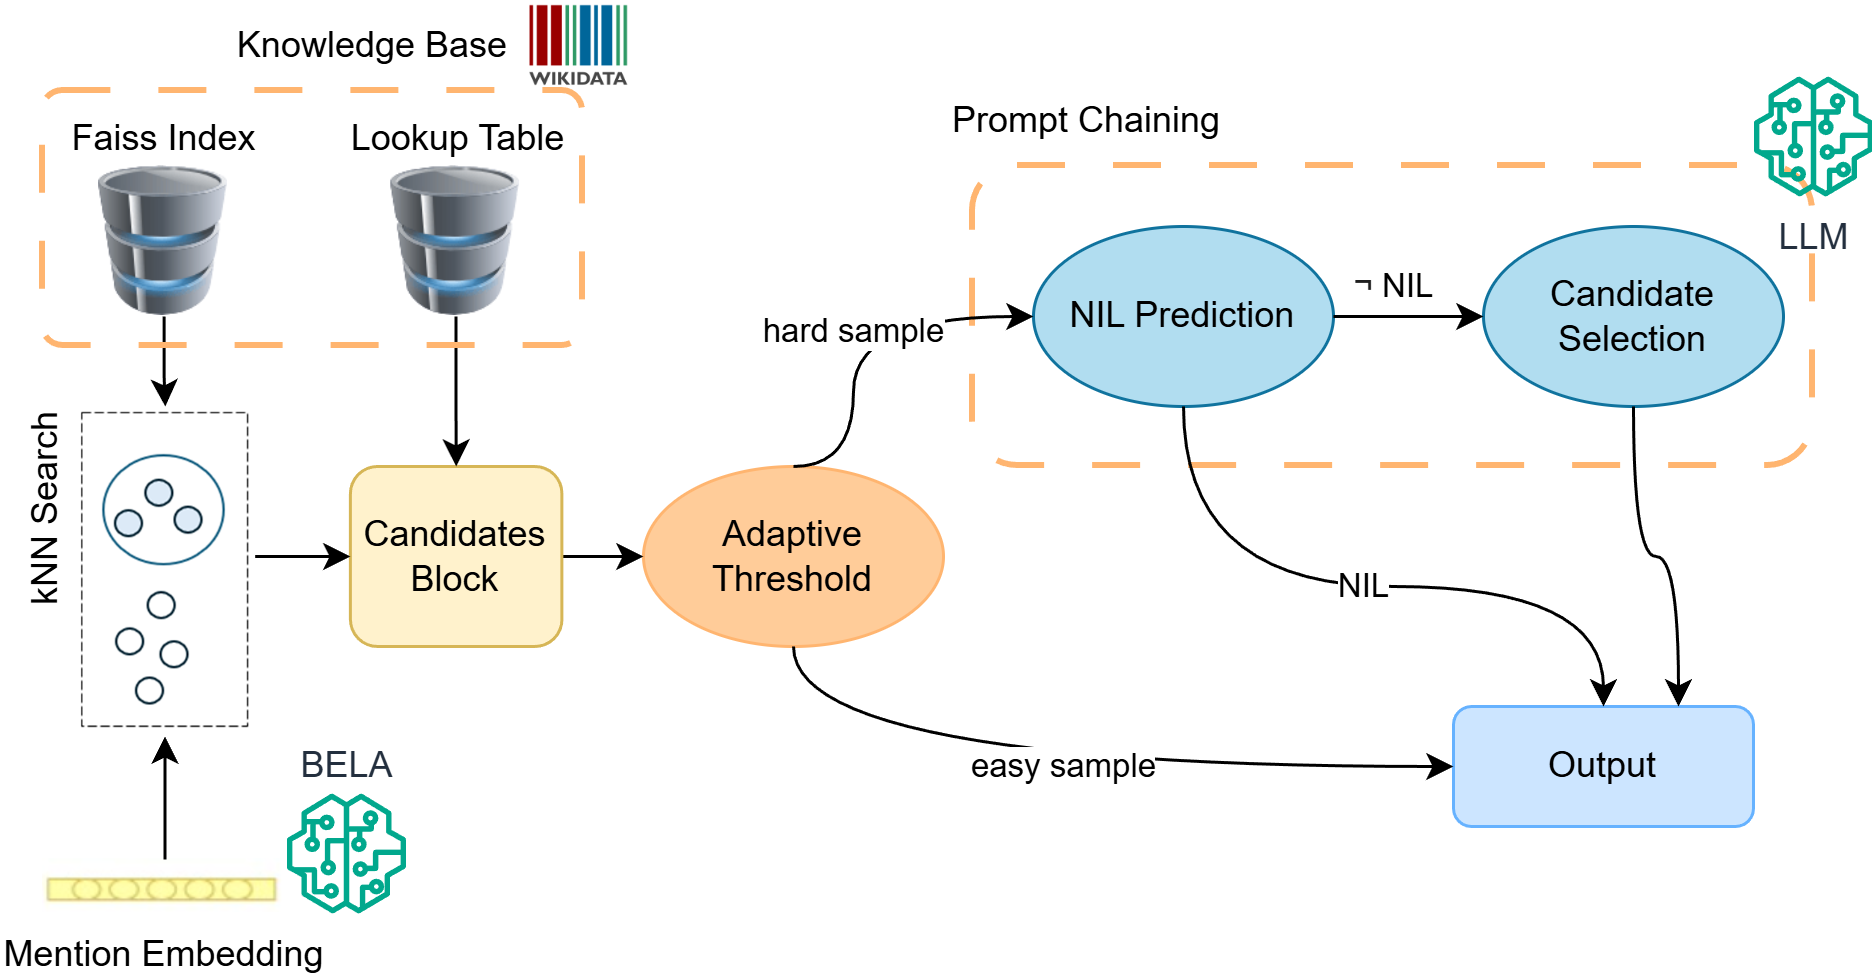
\includegraphics[width=0.85\textwidth]{Figures/mhel_llamo_arch.png}
\caption{MHEL-LLaMo architecture diagram (from repository).}
\label{fig:mhell_arch}
\end{figure}

\begin{lstlisting}[language=Python, caption={Confidence-based routing in MHEL-LLaMo}, label={lst:mhell_route}]
 if bela_confidence >= tau:
     prediction = bela_top1
 else:
     prediction = llm_prompt_chain(mention, candidates)
\end{lstlisting}

\subsection{Retriever Fix and RAG Enhancement}
We fixed a retrieval indexing bug that caused out-of-range errors when invalid mentions were filtered. Listing \ref{lst:valid_idx_fix} shows the corrected logic. We also added a lightweight RAG pipeline with cross-encoder re-ranking and context augmentation to improve difficult cases.

\begin{lstlisting}[language=Python, caption={Valid index tracking in retriever}, label={lst:valid_idx_fix}]
 valid_idx = 0
 for text, length in zip(texts, mention_lengths):
     if length > 0:
         ex_indices = indices[valid_idx]
         ex_scores = scores[valid_idx]
         valid_idx += 1
     predictions.append(candidates)
\end{lstlisting}

\subsection{Threshold Calibration (Beyond Fixed Threshold)}
We replaced the fixed confidence threshold with a dataset-aware calibration step, using development candidate files to search for a threshold that maximizes $F_1$. Listing \ref{lst:threshold_search} shows the core logic used for threshold tuning. This improves robustness across languages by adapting to score distributions rather than relying on a single static value.

\begin{lstlisting}[language=Python, caption={Threshold search for confidence calibration}, label={lst:threshold_search}]
def find_optimal_threshold(data, threshold_range=(0.0, 30.0), num_thresholds=100):
    thresholds = np.linspace(threshold_range[0], threshold_range[1], num_thresholds)
    best_f1, best_threshold = 0.0, 0.0
    for t in thresholds:
        f1, tp, fp, fn = calculate_f1_at_threshold(data, t)
        if f1 > best_f1:
            best_f1, best_threshold = f1, t
    return best_threshold, best_f1
\end{lstlisting}

\subsection{Benchmark Results}
Table \ref{tab:mhell_best} lists the best-setting results from the repository. Figure \ref{fig:mhell_paper_strict} compares the paper score with strict micro-F1, highlighting coverage gaps.

\begin{table}[ht]
\centering
\caption{MHEL-LLaMo best-setting results (reproduced).}
\label{tab:mhell_best}
\begin{tabular}{lccc}
\hline
Dataset & Paper Score & Strict F1 & Coverage \\
\hline
HIPE\_DE & 0.620 & 0.619 & 0.994 \\
HIPE\_EN & 0.723 & 0.708 & 0.960 \\
HIPE\_FR & 0.692 & 0.689 & 0.992 \\
NEWSEYE\_DE & 0.556 & 0.555 & 0.997 \\
NEWSEYE\_FI & 0.509 & 0.490 & 0.928 \\
NEWSEYE\_FR & 0.662 & 0.660 & 0.994 \\
NEWSEYE\_SV & 0.521 & 0.521 & 1.000 \\
AJMC\_DE & 0.521 & 0.509 & 0.955 \\
AJMC\_EN & 0.497 & 0.489 & 0.968 \\
AJMC\_FR & 0.635 & 0.614 & 0.935 \\
MHERCL\_EN & 0.705 & 0.705 & 1.000 \\
MHERCL\_IT & 0.698 & 0.698 & 1.000 \\
\hline
\end{tabular}
\end{table}

\begin{figure}[ht]
\centering
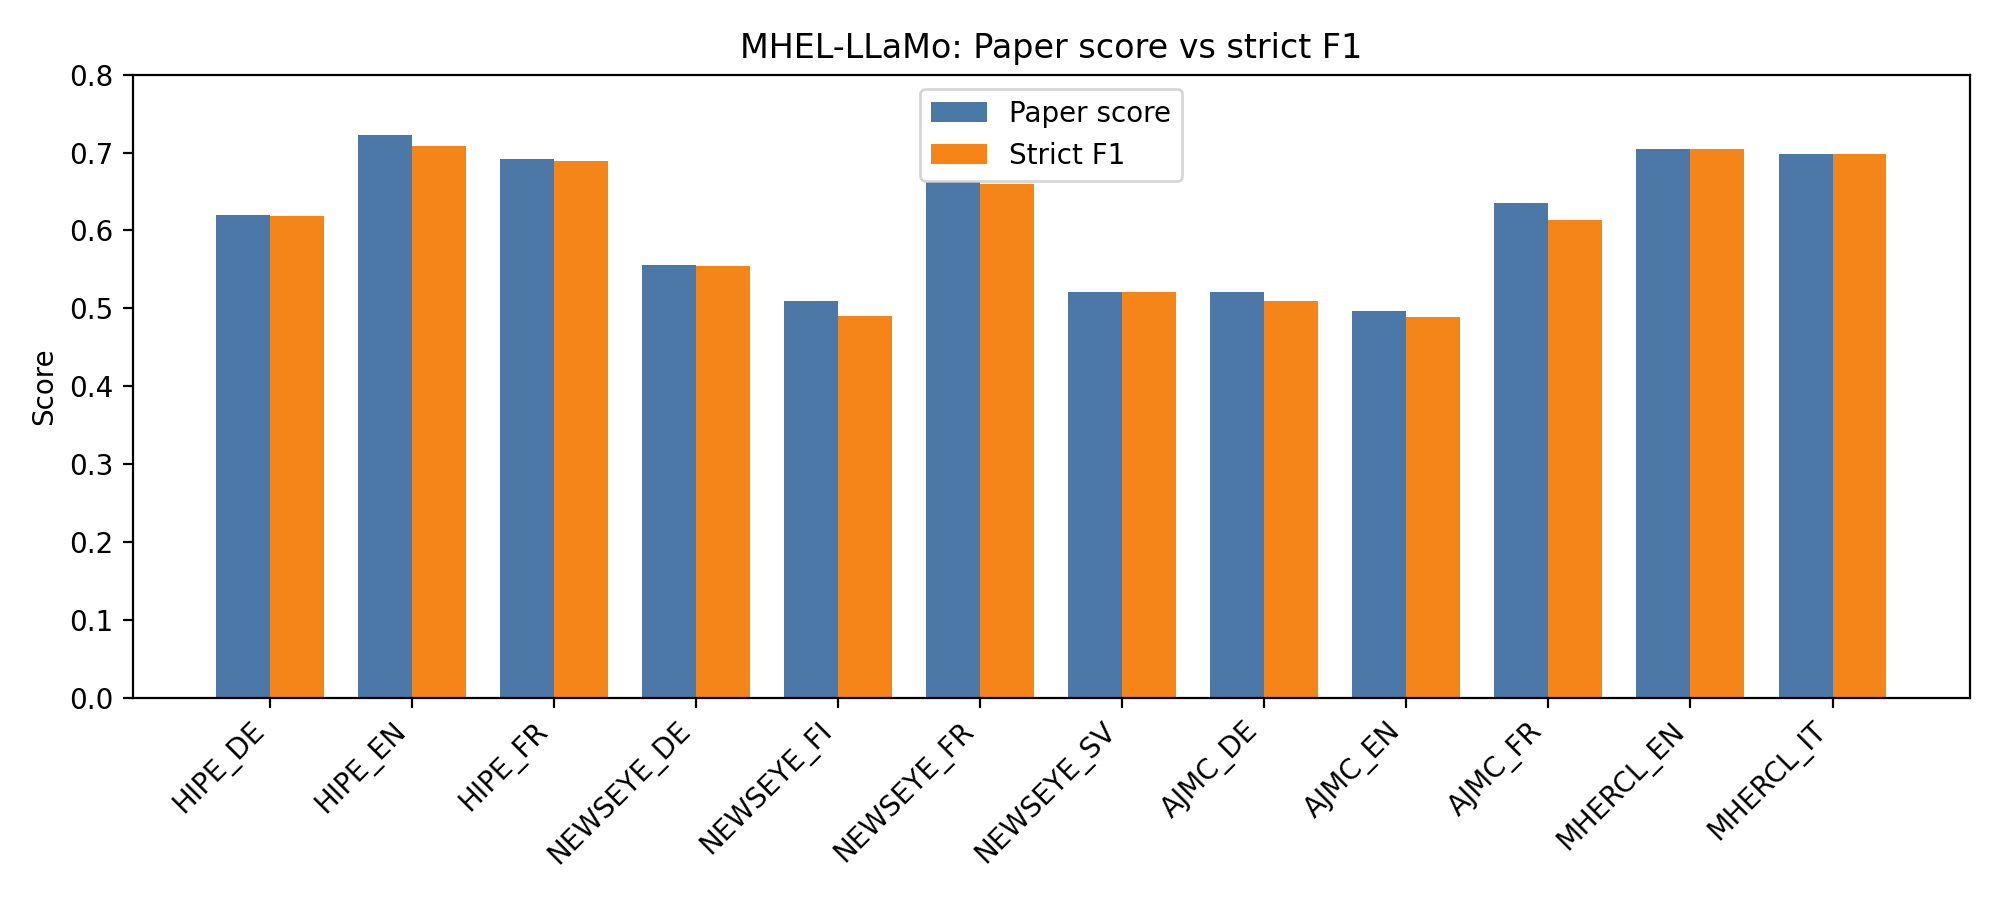
\includegraphics[width=0.9\textwidth]{Figures/mhell_paper_vs_strict.png}
\caption{MHEL-LLaMo: paper score vs strict F1 (reproduced, replotted).}
\label{fig:mhell_paper_strict}
\end{figure}

\section{Summary of Post-Mid Findings}
\begin{itemize}
    \item mReFinED MEWSLI-9 reproduction is feasible with compatibility fixes; disambiguation remains the dominant error source for non-Latin scripts.
    \item TR2016 performance is limited by corrupted mention offsets; offset validation provides measurable recall uplift but does not fully close the gap.
    \item MHEL-LLaMo is robust and reproducible across historical datasets; strict evaluation exposes coverage gaps not visible in legacy metrics.
    \item XGBoost confidence router improves routing accuracy from 70\% (baseline threshold) to 82\% (+12\%), enabling better easy/hard sample discrimination.
    \item Error analysis reveals that short mentions (median 5 chars) and abbreviations (Ph., Ant., El.) are systematic failure modes; these justify the need for LLM routing on borderline cases.
    \item Our primary improvements are engineering-driven: hardware adaptation, model tuning (XGBoost router), threshold calibration, and retrieval pipeline fixes that enable stable, efficient runs under limited resources.
\end{itemize}
